\documentclass[oneside,13pt,a4paper]{article}

% Chargement d'extensions
\usepackage[utf8]{inputenc}
\usepackage[french]{babel}
\usepackage{graphicx}
\usepackage[top=3cm, bottom=3cm, left=3cm, right=3cm]{geometry}
\usepackage{amsmath}
\usepackage{amssymb}

% Liens et autres
\usepackage{hyperref}
\hypersetup{
    colorlinks=true,
    linkcolor=black,
	urlcolor=blue,
	pdftitle={Rendu},
	bookmarks=true,
}

% Bout de code
\usepackage{listings}
\usepackage{color}

\definecolor{mygreen}{rgb}{0,0.6,0}
\definecolor{mygray}{rgb}{0.5,0.5,0.5}
\definecolor{mymauve}{rgb}{0.58,0,0.82}

\lstset{
  backgroundcolor=\color{white},   % choose the background color; you must add \usepackage{color} or \usepackage{xcolor}; should come as last argument
  basicstyle=\footnotesize,        % the size of the fonts that are used for the code
  breakatwhitespace=false,         % sets if automatic breaks should only happen at whitespace
  breaklines=true,                 % sets automatic line breaking
  captionpos=b,                    % sets the caption-position to bottom
  commentstyle=\color{mygreen},    % comment style
  deletekeywords={...},            % if you want to delete keywords from the given language
  escapeinside={\%*}{*)},          % if you want to add LaTeX within your code
  extendedchars=true,              % lets you use non-ASCII characters; for 8-bits encodings only, does not work with UTF-8
  firstnumber=0,                   % start line enumeration with line 1000
  frame=single,	                   % adds a frame around the code
  keepspaces=true,                 % keeps spaces in text, useful for keeping indentation of code (possibly needs columns=flexible)
  keywordstyle=\color{blue},       % keyword style
  %language=C++,                    % the language of the code
  morekeywords={*,...},            % if you want to add more keywords to the set
  numbers=left,                    % where to put the line-numbers; possible values are (none, left, right)
  numbersep=5pt,                   % how far the line-numbers are from the code
  numberstyle=\tiny\color{mygray}, % the style that is used for the line-numbers
  rulecolor=\color{black},         % if not set, the frame-color may be changed on line-breaks within not-black text (e.g. comments (green here))
  showspaces=false,                % show spaces everywhere adding particular underscores; it overrides 'showstringspaces'
  showstringspaces=false,          % underline spaces within strings only
  showtabs=false,                  % show tabs within strings adding particular underscores
  stepnumber=1,                    % the step between two line-numbers. If it's 1, each line will be numbered
  stringstyle=\color{mymauve},     % string literal style
  tabsize=2,	                   % sets default tabsize to 2 spaces
}

% Commande pour notation 'NB :' (nota bene)
\newcommand\nb[1][0.3]{N\kern-#1emB : }

% csquotes va utiliser la langue définie dans babel
\usepackage[babel=true]{csquotes}

% pour afficher Schéma au lieu de figure dans les legende des images
\addto\captionsfrench{\def\figurename{Schéma}}

% Informations le titre, le(s) auteur(s), la date
\title{}
\author{
    Chakib ELHOUITI \and
    Massili KEZZOUL \and
}
\date{\today}


\begin{document}
%\maketitle
\begin{titlepage}
	\centering
	{\scshape\LARGE Universite de Montpellier\par}
	{\scshape\Large\par}
	\vspace{1.5cm}
	{\huge\bfseries Rapport Csp Optimisation\par}
	\vspace{2cm}
	{\Large\itshape
		
		Chakib ELHOUITI \\
		Massili KEZZOUL \\
		
		\par}

		\vspace{2cm}

	\begin{figure}[h]
		\begin{minipage}[c]{.46\linewidth}
			\centering
			
\includegraphics[width=1\textwidth]{img/univ-montpellier.png}
		\end{minipage}
		\hfill%
		\begin{minipage}[c]{.46\linewidth}
			\centering
			
\includegraphics[width=1\textwidth]{img/fds.png}
		\end{minipage}
	\end{figure}

	\par\vspace{1cm}

	\vfill

	% Bottom of the page
	{\large \today\par}
\end{titlepage}





% ------------------------------------- %
% Introduction
% ------------------------------------- %

\parskip=5pt



% Espacement entre les paragraphes
\parskip=5pt
% ------------------------------------- %
% Organisation
% ------------------------------------- %

\section{Introduction}
Ce projet s'attache à mettre en place des optimisations au resolveur de CSP.

Il est demandé de réaliser au moins une des optimisations suivantes : 
- heuristique d'assignation des variables, 
- test de viol de contraintes même si toutes les variables de la contrainte ne sont pas assignées, 
- arc-consistance, 
- forward checking...

Le projet est suivi d'un travail d'évaluation complet des effets des différentes optimisations.


\section {Construction du benchmark}
On a commencé par réaliser un script Python, qui ne permet de construire un benchmark avec des valeurs  de (n,c,d,t) différentes, ce qui veut dire, notre script Python utilise le csp generateur pour generer 10 instance de Networ pour un  niveau de dureté (1--100) en les stockant dans des fichiers sous un format bien précis(ex: d1-I7.txt), pour pouvoir aprés automatiser la tache d'execution pour notre APP java. 
\subsection{}

\section{Implementation des optimisations}
Dans notre cas on a pu réaliser deux optimisations : 
\subsection{Forward Cheking}

On a réalisé l'implémentation de l'algorithme Forward Cheking, pour pouvoir remplacer backtrack.
\subsubsection{Resultats du Forward Cheking }
On a pu constaté en variant les differents Valeur pour generer un réseau de contrainte aléatoire et sur un niveau de dureté de 1 à 100. L'algo du forward cheking permet en premier lieu de resoudre les réseaux de grande taille en fonction de (n,c,d,t).

Concernant le graphe obtenu pour une execution de réseaux de contrainte pour des niveaux de dureté de 1 à 100, on a calculé le temps moyen de 5 execution par instance, on a obtenu : un graph avec un temps élevé, c'est du à l'algo du forward cheking (plus de tuples avec plus de contraintes = plus de temps). Concernant la phase de transition, on remarque bien un pic pour le temps moyen par dureté
Ce qui montre le graphe  suivant : (n = 35, c=249, d = 17 et le t est calculé)

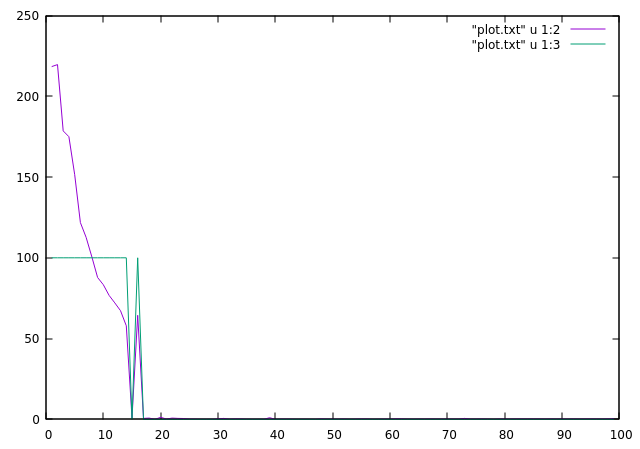
\includegraphics{img/FC.png}


\subsection{L'heuristique MaxDegré}

Pour cette heuristique, on a commencé par stocker une Hashmap (string,int) qui permet de stocker les variables du réseau avec leurs nombre d'occurences dans les contraintes (le degré), ensuite on tri cette HashMap par ordre décroissant et on choisi a chaque fois la variable qui n'est pas assignée avec le plus grand degré.
\subsubsection{Resultats du maxDegré}
Cette heuristique ne permet pas de résoudre des CSP avec de grande taille comme il le fait FC, mais permet bien de constater à travers un graphe le pic lors de la phase de transition.
Elle reste toujours meilleure que le backtrack avec chooseVar sans aucune heuristique mais performante que le forward cheking.

exemple de graphe : (n = 20, c=50 , d = 17)

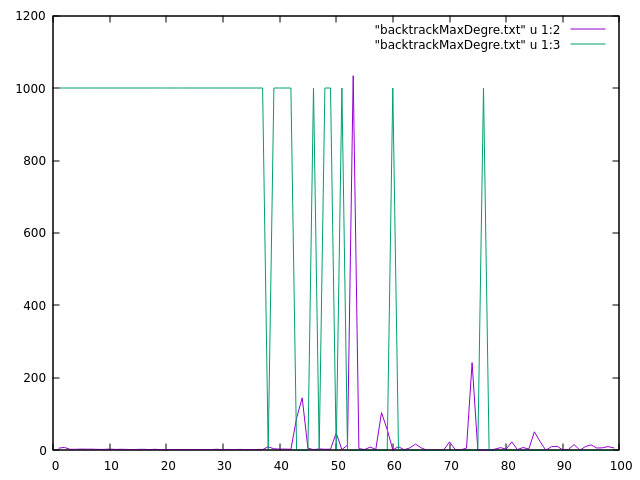
\includegraphics{img/backtrackMaxDegre.png}

\subsection{Exécution des programmes}
pour éxecuter le programme il suffit de :
\begin{itemize}	
	\item Ouvrire un terminal et se rendre au dossier src/
	\item Ajouter les droits d'éxecutions au programme exec.sh
	\item Puis l'éxecuter `exec.sh`
\end{itemize}

Le script génère un benchmark puis éxecuter l'algorithme de résolution sur ce dernier et gnuplot sur le resultat. Vous aurez donc à la fin un fichier graphe.png qui contient la courbe du temps d'éxecution ainsi que le tracé de transition de phase.

\section{materiels et systèmes : }
On a utilisé deux script dans notre implementation, le premier en Python pour générer les fichiers de tests et le deuxiéme en Shell pour automatiser l'exécution.
\begin{itemize}
	\item Processeur : Comme on est deux, on testé avec un I5 7ème génération et un I5 2ème génération, on a remarqué une petite différence sur le temps moyen mais les résultats étaient les mêmes.
	\item Ram : 8GB et 4GB
	\item OS : Pop'Os (20.04) c'est une distribution Linux similaire à ubuntu mais plus stable (à notre avis).
	\item Compilateur : Javac 11.0.9
\end{itemize}

\end{document}
